\chapter{建立整篇论文的视觉语言}

海洋科学博士生小宋正在准备一篇综述论文的投稿定稿。论文利用四套公开观测与碳收支数据集，梳理“全球海洋如何吸收气候系统中的新增热量与人为排放的二氧化碳（$\text{CO}_2$）”。全文共有四张配图：图 1 是海气界面热量与碳吸收主要途径的概念示意图；图 2 展示夏威夷莫纳罗亚（Mauna Loa）站大气 $\text{CO}_2$ 浓度，以及北太平洋 ALOHA 站表层海水二氧化碳分压（$p\text{CO}_2$）与 pH 的长期变化；图 3 展示全球海洋 $0\text{--}700\ \text{m}$ 与 $0\text{--}2000\ \text{m}$ 水层热含量距平的时间序列；图 4 展示全球人为 $\text{CO}_2$ 排放的去向（大气增长、海洋碳汇、陆地碳汇）及海洋碳汇占总排放的比例。

这四张图是在两个月里陆续画完的：图 1 用图像生成工具出图，图 2 至图 4 分别在不同日期用脚本或对话式工具生成。单看任何一张似乎都说得过去，但提交前导师让小宋把四张图缩印在同一张 A4 纸上并排审读（图~\ref{fig:ch04-01}），问题立刻暴露无遗——审稿人后来也给出了同样的意见：“各图之间难以对照，颜色与符号含义前后冲突。”

\begin{figure}[htbp]\centering
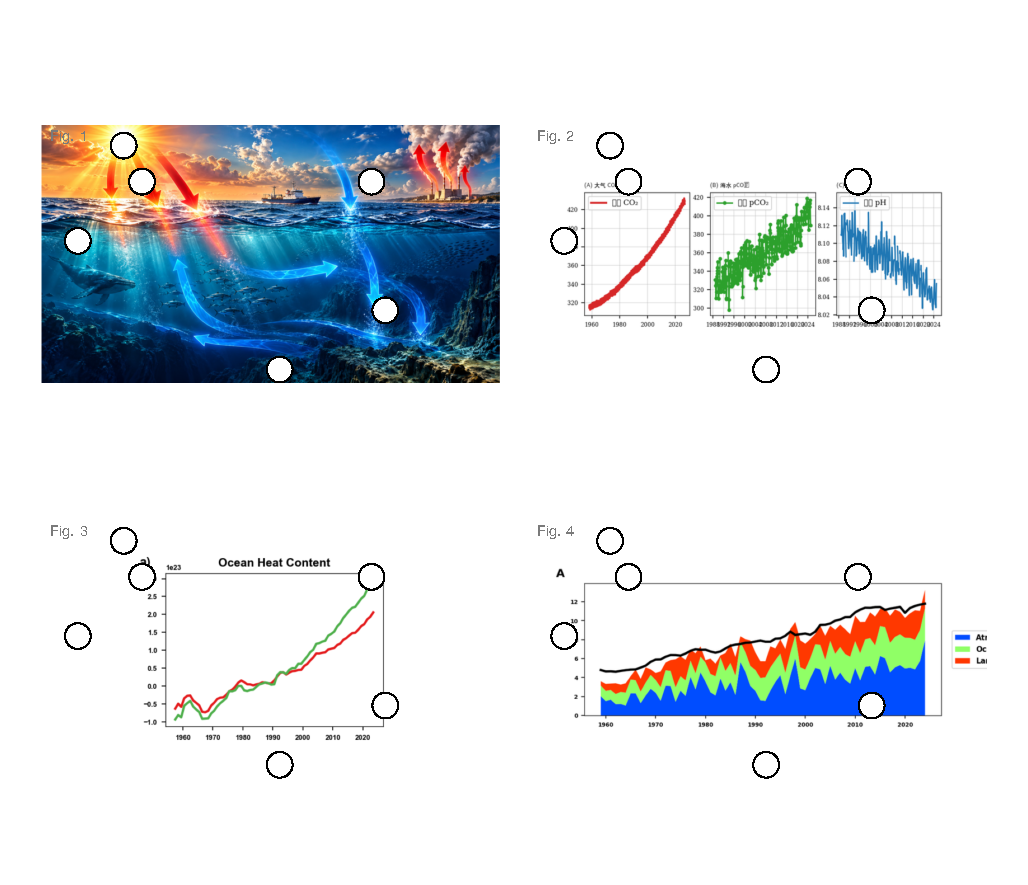
\includegraphics[width=\linewidth]{figures/ch04/ch04-01-inconsistent-set-zh.pdf}
\caption{四张各自看来都还可以的图，放在一起却不成一套（故意不一致的示范）。图中存在六类冲突：（1）红色在四张图中分别表示太阳辐射与工厂排放（Fig.\ 1）、大气 $\text{CO}_2$（Fig.\ 2）、$0\text{--}700\ \text{m}$ 海洋热含量（Fig.\ 3）和陆地碳汇（Fig.\ 4）；（2）示意图中同色箭头兼表不同过程；（3）Fig.\ 3 仅靠红绿区分两条线且未标图例；（4）Fig.\ 4 用彩虹色图绘制堆叠面积，右侧图例被裁切；（5）四图混用三种字体与四种面板编号写法，且因字体未统一配置，子图标题与标记圆圈中的上下标或序号出现缺字方框与空白圆圈；（6）示意图采用立体光泽画风，并混入太阳、轮船、鲸、鱼群等正文未讨论的对象。Fig.\ 2–4 使用真实公开数据，仅改变了样式。}\label{fig:ch04-01}
\end{figure}

顺着读者的视线在图~\ref{fig:ch04-01} 的四个象限间扫视，就能体会读图的阻力：左上角 Fig.\ 1 中，发光红箭头既从太阳射向海面（热量输入），又从工厂烟囱升向天空（人为碳排放）；右上角 Fig.\ 2 中，红线代表大气 $\text{CO}_2$；左下角 Fig.\ 3 中，红线变成 $0\text{--}700\ \text{m}$ 海洋热含量；右下角 Fig.\ 4 中，顶层红色色块又变成陆地碳汇。绿色在 Fig.\ 2b、Fig.\ 3、Fig.\ 4 中分别代表海水 $p\text{CO}_2$、$0\text{--}2000\ \text{m}$ 热含量和海洋碳汇；蓝色在 Fig.\ 1、Fig.\ 2c、Fig.\ 4 中分别代表海气交换与环流、海水 pH 和大气碳增长。读者每翻过一张图，都得强行忘掉上一张图的颜色含义，重新寻找图例解码（表~\ref{tab:ch04-diag}）。

\begin{table}[htbp]\centering\footnotesize
\setlength{\tabcolsep}{3pt}
\renewcommand{\arraystretch}{1.15}
\caption{不一致初稿（图~\ref{fig:ch04-01}）的逐项诊断及其给读者造成的理解代价。}\label{tab:ch04-diag}
\begin{tabularx}{\linewidth}{@{}Y>{\raggedright\arraybackslash}p{18mm}Y@{}}
\toprule
\textbf{初稿中出现的视觉冲突} & \textbf{出现位置} & \textbf{读者付出的理解代价} \\
\midrule
红、绿、蓝三色跨图含义冲突（如红色在四图中分别代表热与排放、大气 $\text{CO}_2$、上层热含量、陆地碳汇） & Fig.\ 1–4 & 读者在图间来回对照时，误把同一颜色当成同一个物理量或碳库 \\
示意图中蓝色箭头既表示水体环流又表示海气碳交换，红色箭头既表示太阳热辐射又表示烟囱碳排放 & Fig.\ 1 & 无法从箭头的几何外观判断所代表的过程类型 \\
仅靠纯红与纯绿区分两条等粗曲线，且图面未标图例或直接标注 & Fig.\ 3 & 红绿色觉差异读者无法分辨 $0\text{--}700\ \text{m}$ 与 $0\text{--}2000\ \text{m}$ 深度层 \\
采用 \texttt{jet} 彩虹色图绘制三层碳汇堆叠面积，且因未画收支不平衡项导致堆叠顶缘穿越总排放黑线 & Fig.\ 4 & 颜色顺序无物理意义，明度跳跃制造假边界，且造成“分项之和大于总排放”的误读 \\
混用三种字体与四种面板编号格式（\texttt{(A)}、\texttt{a)}、\texttt{A}、无编号），上下标与圆圈序号出现缺字方框 & Fig.\ 1–4 & 版面显得临时拼凑；正文引用“图 3a”或“图 2b”时读者难以快速定位 \\
字号从 $6\ \text{pt}$ 到 $12\ \text{pt}$ 不等，图内标题与下方图注重复，右侧图例框超出画布被裁切 & Fig.\ 2–4 & 视觉层级混乱，挤占数据展示面积，且产生残缺文字 \\
3D 立体光泽示意图与二维扁平数据图风格割裂，示意图中加入太阳、轮船、鲸和鱼群 & Fig.\ 1 & 暗示正文并未讨论的短波辐射或生态航次过程，视觉重心落在装饰物上 \\
纵轴单位记法不一，Fig.\ 3 因重复乘上量级因子触发顶端“\texttt{1e23}”科学计数偏移且无单位名称 & Fig.\ 2–4 & 读者需要停下来重新换算数量级与物理量纲 \\
\bottomrule
\end{tabularx}
\end{table}

一篇论文的所有配图不是孤立插画，而是一套协同论证的视觉系统。当多个面板反复讨论同一批物理量或碳库时，颜色、字号、线型、箭头和图标就构成了整篇论文的\textbf{视觉语言}。本章讨论如何在动手出图前立下一页视觉规范，将其转化为可粘贴进 \scidraw{} 的风格约束与核验清单，让全篇配图讲同一种语言。

\section{颜色先有含义，再有好看}

许多研究者配色时首先关心“哪套色板更好看”。但在科研论文中，颜色的首要职责不是装饰，而是\textbf{承载语义}。读者会本能地把同一种醒目颜色当成同一研究对象或同一类物理量（Wong, 2010；Krzywinski, 2013）。若颜色只按单张图的作图顺序随意分配，跨图对照的线索就会断裂。

\textbf{第一，按科学含义分配“语义色”，并在全文锁定。}建立视觉语言的第一步，是列出全文所有图表中反复出现的核心物理量或角色，为每个角色指定专属色值（语义色），明确规定它“用于什么”和“绝不用于什么”。在小宋的论文中，全文锁定六个定量角色与一个示意图专用角色：
\begin{itemize}
\item \textbf{大气碳（$\text{CO}_2$）：}橙色（\texttt{\#E69F00}），用于 Fig.\ 1 大气 $\text{CO}_2$ 分子点、Fig.\ 2a 大气 $\text{CO}_2$ 曲线和 Fig.\ 4a 大气碳增长，不用于热量或海洋量。
\item \textbf{海洋碳：}蓝色（\texttt{\#0072B2}），用于 Fig.\ 1 表层海水溶解无机碳（DIC）、Fig.\ 2b 海水 $p\text{CO}_2$、Fig.\ 4a 海洋碳汇及 Fig.\ 4b 海洋碳汇占比，不用于水体背景或温度。
\item \textbf{陆地碳：}蓝绿色（\texttt{\#009E73}），仅用于 Fig.\ 4a 陆地碳汇，不用于示意图中的浮游植物图标。
\item \textbf{热量：}朱红色（\texttt{\#D55E00}），用于 Fig.\ 1 热通量箭头和 Fig.\ 3 海洋热含量曲线，不用于任何碳量。
\item \textbf{海水 pH：}红紫色（\texttt{\#CC79A7}），专用于 Fig.\ 2c 表层海水 pH。
\item \textbf{人为排放与碳输入通量：}近黑深灰（\texttt{\#3C3C3C}），用于 Fig.\ 4a 总排放曲线及 Fig.\ 1 碳通量方向箭头。
\item \textbf{水体输运（仅示意图）：}天蓝色（\texttt{\#56B4E9}）半透明宽带，专用于 Fig.\ 1 携热与碳下沉的环流带，不作数据图折线。
\end{itemize}

\textbf{第二，控制语义色总数，用同色相的不同明度区分同类变体。}人眼在同一视野内无需反复查表即可记住的颜色类别很有限，全文语义色不宜超过 6 至 7 个（Wong, 2010）。坐标轴、参考线、背景分区和示意图标本体一律退居中性灰（\texttt{\#F2F2F2}、\texttt{\#BDBDBD}、\texttt{\#7A7A7A}）。当同一面板需比较同一物理量的两个变体——如 Fig.\ 3 同时展示 $0\text{--}700\ \text{m}$ 与 $0\text{--}2000\ \text{m}$ 海洋热含量距平——不应借用代表碳汇的绿或蓝，而应\textbf{保持“热量 = 朱红（\texttt{\#D55E00}）”的色相不变，用深浅明度区分深度}：$0\text{--}2000\ \text{m}$ 用全饱和度深朱红（\texttt{\#D55E00}），$0\text{--}700\ \text{m}$ 用向白色混合 $45\%$ 的浅朱红（保留 $55\%$ 原色强度），并在曲线右端直接标出深度（图~\ref{fig:ch04-02}、图~\ref{fig:ch04-03}）。读者一眼便知两条线都代表海洋热量，又能清晰分辨深浅两层。

\begin{figure}[htbp]\centering
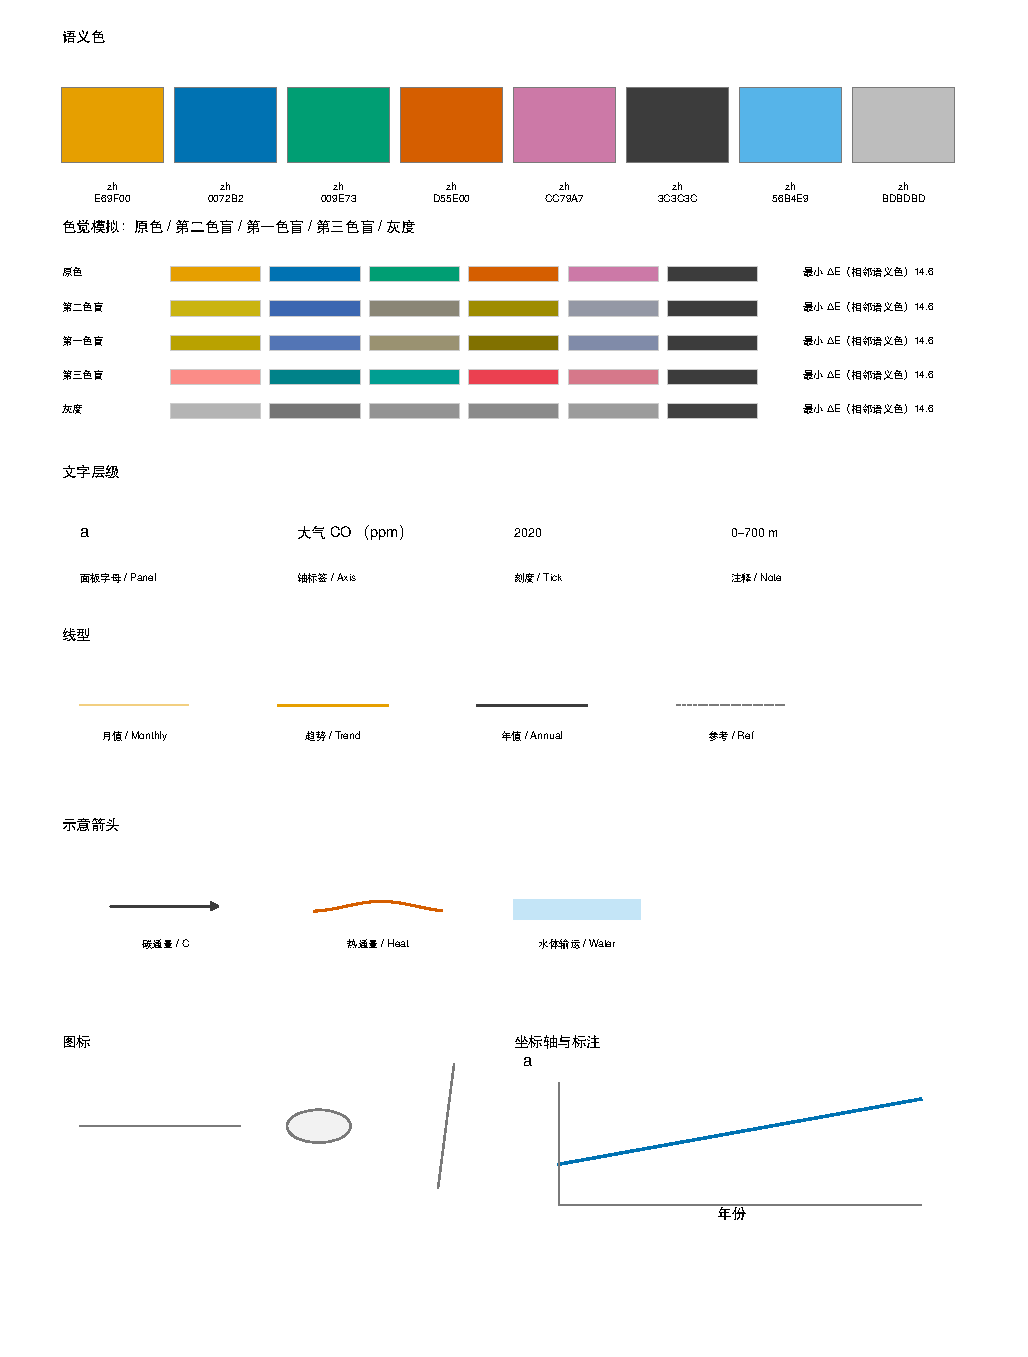
\includegraphics[width=0.95\linewidth,height=0.80\textheight,keepaspectratio]{figures/ch04/ch04-02-spec-page-zh.pdf}
\caption{本案例论文的一页视觉规范（v1）。自上而下规定语义色色板、三种色觉差异模拟与灰度检查、最终印刷尺寸下的四级文字层级、数据图线型、示意图过程箭头、中性图标风格及坐标轴布局。色觉模拟行右侧数值（$14.6$）为同面板相邻语义色间的最小感知色差（CAM02-UCS $\Delta E$），由脚本计算。}\label{fig:ch04-02}
\end{figure}

\textbf{第三，以无障碍色板为起点，绝不单靠红绿区分。}欧洲血统人群中约 $8\%$ 的男性存在先天性红绿色觉差异，其中以第二色觉异常（deuteranomaly，绿色弱/盲）最常见（Wong, 2011；注意该文于 2023 年发表了作者更正，修正了原文视锥细胞光谱曲线标注与部分术语）。图~\ref{fig:ch04-01} 中 Fig.\ 3 纯靠鲜红（\texttt{\#E41A1C}）与鲜绿（\texttt{\#4DAF4A}）区分的两条等粗曲线，在第二色盲模拟下会变成两条难以分辨的暗黄褐色线（图~\ref{fig:ch04-03} 上行右列）。因此，选色应以经过色觉通用设计验证的 Okabe–Ito 色板（Okabe 与 Ito, 2008；Wong, 2011）或 ColorBrewer 方案（Brewer）为起点。

\begin{figure}[htbp]\centering
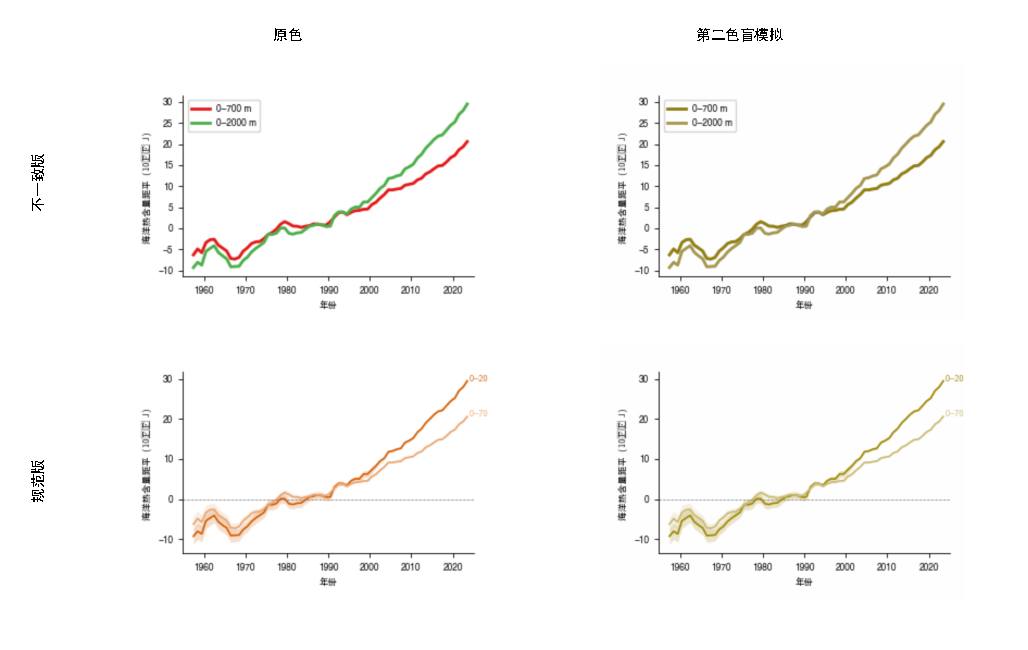
\includegraphics[width=\linewidth]{figures/ch04/ch04-03-cvd-check-zh.pdf}
\caption{只靠红绿区分的两条线，在第二色盲模拟下难以分辨（上）；同一色相的两种明度加直接标注，在模拟下仍可区分（下）。右列为对整幅渲染图像像素执行的第二色盲模拟（\texttt{colorspacious}，deuteranomaly，严重度 $100$）。数据：NOAA NCEI 全球海洋热含量五年平均距平（Levitus 等, 2012）。}\label{fig:ch04-03}
\end{figure}

\textbf{第四，结合色觉模拟与灰度检查，叠加冗余编码。}即便选用 Okabe–Ito 色板，多色同框时仍需定量核验。图~\ref{fig:ch04-02} 第二部分展示了各语义色在原色、第二色盲、第一色盲（protanomaly）、第三色盲（tritanomaly，严重度均为 $100$）及 CIELAB 明度灰度（$L^*$）下的外观，并计算同面板相邻语义色在 CAM02-UCS 空间中的最小色差 $\Delta E$。本书给出一条操作建议（属于实用自查参考值，非强制标准）：\textbf{同面板相邻颜色在色觉模拟下的 CAM02-UCS 色差宜满足 $\Delta E \ge 15$，转灰度后的明度差宜满足 $\Delta L^* \ge 15$；若不足，则必须叠加形状、线型或线端直接标注作为冗余。}

图~\ref{fig:ch04-02} 中相邻语义色的最小 $\Delta E$ 实测值为 $14.6$，刚巧擦过 $15$ 的参考线边缘，且灰度行中蓝、蓝绿与朱红的明度颇为接近。这说明任何多色色板都不能单靠色相硬扛。如图~\ref{fig:ch04-03} 下行所示，改用深浅朱红配标准误阴影带与右端直接标注后，即使在严重度 $100$ 的第二色盲模拟下依然清晰可辨。同时需注意，数值模拟只是色度学近似，定稿前打印黑白稿自查并请有色觉差异的同行看一眼，不能省略。

\textbf{第五，连续变量用感知均匀色图，告别彩虹色图。}映射二维连续场或多项堆叠时，禁用 \texttt{jet} 等彩虹色图。Crameri 等（2020）指出，彩虹色图明度随数值变化不单调，在青、黄区制造虚假边界且对色觉差异读者不友好。连续单向变量应选 \texttt{viridis} 或 \texttt{cividis}（Nuñez 等, 2018）等感知均匀顺序色图；正负距平应以零值为中心选用双端发散色图。

\section{文字层级按最终尺寸定}

图~\ref{fig:ch04-01} 显得拼凑的另一原因是文字失控：Fig.\ 2 用衬线体 \texttt{DejaVu Serif}（$11\ \text{pt}$）、编号“\texttt{(A)(B)(C)}”；Fig.\ 3 用 \texttt{Arial} 粗体（$9\ \text{pt}$）、编号“\texttt{a)}”；Fig.\ 4 用 \texttt{DejaVu Sans}（$8\ \text{pt}$）、编号“\texttt{A}”。各图画布尺寸不一，缩进论文版心后字号忽大忽小。

\textbf{第一，先锁定期刊最终印刷尺寸，再定字号。}若在脚本里随手设 $10 \times 6$ 英寸（约 $254 \times 152\ \text{mm}$），缩进单栏宽 $85\ \text{mm}$ 时字号会缩至三分之一，$10\ \text{pt}$ 刻度变成难以辨认的 $3.3\ \text{pt}$（Rougier 等, 2014；Wong, 2011 Typography）。正确顺序是先按目标期刊《作者指南》设定画布物理宽度——单栏图通常宽 $85\text{--}89\ \text{mm}$，双栏通栏图通常宽 $174\text{--}183\ \text{mm}$（本案例 Fig.\ 1、2、4 设为 $174\ \text{mm}$，Fig.\ 3 设为 $85\ \text{mm}$）——再按目标点数设定字号，并在 $100\%$ 打印比例下核对。

\textbf{第二，建立四级文字层级，全文统一无衬线字体。}图面文字靠字号与字重分为四级（图~\ref{fig:ch04-02}“文字层级”区）：
\begin{enumerate}
\item \textbf{面板字母（8 pt 粗体）：}小写粗体 \textbf{a}、\textbf{b}、\textbf{c}，不加括号，置于坐标轴框左上外侧。
\item \textbf{坐标轴标签（7 pt 常规）：}“物理量名称（单位）”，如“大气 $\text{CO}_2$（ppm）”。
\item \textbf{刻度数字（6 pt 常规）：}水平排列，不旋转、不重叠。
\item \textbf{图内注释与示意标签（6–7 pt 常规）：}曲线末端直接标注及状态注记用 $6\ \text{pt}$（曲线标注与曲线同色）；示意图叠加标签中，分区与主要对象用 $7\ \text{pt}$，过程名称用 $6\ \text{pt}$。
\end{enumerate}

英文版全文统一用无衬线体（\texttt{Helvetica}、\texttt{Arial} 或 \texttt{TeX Gyre Heros}），在小字号下笔画均匀清晰（Wong, 2011 Typography）。中文版汉字用等线/黑体（如 \texttt{FandolHei} 或思源黑体），但数字、拉丁字母与单位仍用西文无衬线字体。

这里要警惕一个实测字体陷阱：观察图~\ref{fig:ch04-01} 右上 Fig.\ 2、图~\ref{fig:ch04-02} 文字示例以及后文图~\ref{fig:ch04-05}、图~\ref{fig:ch04-07} 的纵轴标签可见，当脚本把 Unicode 下标 $2$、上标负号或带圈序号直接混在中文字符串里交给黑体渲染时，由于中文字库缺少这些专用字形，PNG 栅格图中出现了缺字方框，而在走 PGF/XeLaTeX 的 PDF 中缺字被静默丢弃——导致“大气 $\text{CO}_2$”变成“大气 CO”、“$\text{GtC yr}^{-1}$”变成“$\text{GtC yr}^{1}$”，图~\ref{fig:ch04-02} 色块上方也因脚本元组索引错位印出了语言代码“\texttt{zh}”。因此，混排中英文与上下标时不能依赖字体自动回退，应使用规范的数学/上下标语法（如 \texttt{\textbackslash textsubscript\{2\}}），并在导出 PDF 后放大到 $200\%$ 逐字检查。

\textbf{第三，统一单位记法，用直接标注取代图例框，删去图内标题。}图~\ref{fig:ch04-01} 的 Fig.\ 3 因把已按 $10^{22}\ \text{J}$ 计的数值又乘上 $10^{22}$，触发了纵轴顶端的科学计数偏移“\texttt{1e23}”，且无轴名称。规范做法是全文统一括号内 SI 单位（$10^{22}\ \text{J}$、$\text{GtC yr}^{-1}$、$\mu\text{atm}$、ppm）；删去与图注重复的图内标题；省去图例框，直接把序列名称用同色文字标在曲线右端（Wong, 2011 Typography）。

\section{线型与箭头只说一件事}

在不一致初稿（图~\ref{fig:ch04-01}）中，几何线条同样混乱：Fig.\ 2a 把月均值与去季节趋势画成两条等粗（$2\ \text{pt}$）红线叠成粗带；Fig.\ 2b 用绿实线把离散航次采样点连成折线；Fig.\ 1 示意图用同一种发光粗箭头兼表气体交换、辐射传热和大洋环流。核心原则只有一条：\textbf{同一含义只用一种画法，同一画法只代表一种含义。}

数据图中，不同统计性质或采样频率的数据序列通过线宽、透明度和点线形式严格区分（表~\ref{tab:ch04-lines}）：

\begin{table}[htbp]\centering\footnotesize
\setlength{\tabcolsep}{4pt}
\renewcommand{\arraystretch}{1.15}
\caption{本案例数据图的线型与点型规范（对应视觉规范 C 节）。}\label{tab:ch04-lines}
\begin{tabularx}{\linewidth}{@{}>{\raggedright\arraybackslash}p{36mm}Y>{\raggedright\arraybackslash}p{42mm}@{}}
\toprule
\textbf{数据序列性质} & \textbf{规定画法} & \textbf{本案例应用面板} \\
\midrule
高频原始观测（月均值） & $0.5\ \text{pt}$ 细实线，序列语义色向白色混合 $50\%$ 后的浅色 & Fig.\ 2a 莫纳罗亚大气 $\text{CO}_2$ 月均值 \\
去季节 / 滑动平均趋势 & $1.2\ \text{pt}$ 粗实线，全饱和度语义色 & Fig.\ 2a 去季节值、Fig.\ 3 热含量、Fig.\ 4b 滑动平均 \\
离散航次或非连续采样 & 直径 $2.5\ \text{pt}$ 实心圆点，\textbf{不加连线} & Fig.\ 2b 海水 $p\text{CO}_2$、Fig.\ 2c pH、Fig.\ 4b 年比值 \\
年度收支时间序列 & $1.0\ \text{pt}$ 实线，对应语义色 & Fig.\ 4a 排放与三大碳汇年值 \\
不确定性区间（标准误等） & 同色 $20\%$ 不透明度填充带，无边线 & Fig.\ 3（$\pm 1\ \text{WOse}$）、Fig.\ 4a（平均误差带） \\
参考线与站点变更标记 & $0.5\ \text{pt}$ 中深灰（\texttt{\#7A7A7A}）细虚线，配 $6\ \text{pt}$ 灰字注记 & Fig.\ 2a 换站竖线、Fig.\ 3 零距平水平线 \\
\bottomrule
\end{tabularx}
\end{table}

例如，莫纳罗亚月均值来自连续日观测汇总，用 $0.5\ \text{pt}$ 浅橙细线衬底、叠 $1.2\ \text{pt}$ 鲜橙去季节粗线，既保留季节振幅又突出长期趋势；而夏威夷海洋时间序列（HOT）ALOHA 站数据来自离散出海航次（间隔不均且偶有缺测），若用直线相连就暗示航次之间呈线性变化，因此必须画成无连线圆点。

在概念示意图（Fig.\ 1）中，我们也按“一义一形”为四类物理与生物地球化学过程规定了互不重叠的箭头几何形态（表~\ref{tab:ch04-arrows}）：

\begin{table}[htbp]\centering\footnotesize
\setlength{\tabcolsep}{4pt}
\renewcommand{\arraystretch}{1.15}
\caption{本案例示意图的过程箭头规范（对应视觉规范 D 节）。}\label{tab:ch04-arrows}
\begin{tabularx}{\linewidth}{@{}>{\raggedright\arraybackslash}p{36mm}Y>{\raggedright\arraybackslash}p{44mm}@{}}
\toprule
\textbf{物理 / 生物地球化学过程} & \textbf{规定几何形态与颜色} & \textbf{形状与颜色双重冗余作用} \\
\midrule
碳通量（人为排放、海气交换） & 直线、实心三角头，近黑深灰（\texttt{\#3C3C3C}），$1.0\ \text{pt}$ & 与热通量既靠“深灰对朱红”区分，又靠“直线实心头对波浪开口头”区分 \\
热通量（海气热量吸收与下传） & 波浪线、开口 V 形头，朱红色（\texttt{\#D55E00}），$1.0\ \text{pt}$ & 借用传热学波浪线惯例，黑白打印或色盲视图下仍可凭形状认出 \\
水体下沉与大洋内部输运 & 宽 $4\text{--}6\ \text{pt}$ 天蓝（\texttt{\#56B4E9}）半透明流带，内嵌顺流向人字纹 & 用面状宽带代表大尺度水团运动，与代表界面通量的细线箭头分开 \\
下沉有机颗粒（生物泵输出） & 点线、小实心三角头，近黑深灰（\texttt{\#3C3C3C}），$0.8\ \text{pt}$ & 用离散点线呼应颗粒沉降，线宽细于海气交换主箭头以体现次级角色 \\
\bottomrule
\end{tabularx}
\end{table}

每种箭头在示意图底部图例中定义一次，即使黑白打印，直线、波浪线、人字纹宽带和细点线也绝不会混淆。

\section{图标与示意元素的风格}

在同时包含示意图与数据图的论文里，常见毛病是数据图扁平克制，Fig.\ 1 却是带镜头光晕、水面焦散和立体阴影的 3D 渲染画（图~\ref{fig:ch04-04} 左）。要让示意图融入全文视觉语言，需遵守五条规则（规范 E 节）：

\textbf{第一，图标本体用中性色填充，把语义色留给被追踪的“量”。}工厂烟囱和浮游植物细胞只是过程载体。若把浮游植物涂成绿色，读者就会联想到 Fig.\ 4 的“陆地碳汇（\texttt{\#009E73}）”。因此图标本体一律用浅灰或中灰填充（\texttt{\#F2F2F2}、\texttt{\#BDBDBD}），只让大气 $\text{CO}_2$ 圆点用橙色、表层海水 DIC 圆点用蓝色、热通量箭头用朱红、水体输运带用天蓝；背景水层仅用极低饱和度的浅蓝灰（表层混合层 \texttt{\#DCEBF5}、海洋内部 \texttt{\#C9DEEE}）做结构分层。

\textbf{第二，描边粗细与数据图坐标轴对齐。}数据图坐标轴为 $0.6\ \text{pt}$，示意图标轮廓与海面分界线统一设为接近的 $0.75\ \text{pt}$ 深灰（\texttt{\#3C3C3C}）圆角描边。

\textbf{第三，采用二维简化轮廓，去掉渐变、阴影、高光与写实水纹。}留出干净背景安放文字标签。

\textbf{第四，同一对象在不同图中画法一致。}如海面波线与混合层分界在各处保持相同轮廓。

\textbf{第五，不画未讨论的装饰对象，守住机制表述的科学边界。}图~\ref{fig:ch04-04} 左图画了烈日与直射光束（暗示研究短波辐射）、科考船（暗示特定航次观测），模型还自行生成了鲸、鱼群与海底礁石。这些无关元素会误导读者对研究范围的判断。

\begin{figure}[htbp]\centering
\begin{minipage}[c]{0.48\linewidth}\centering
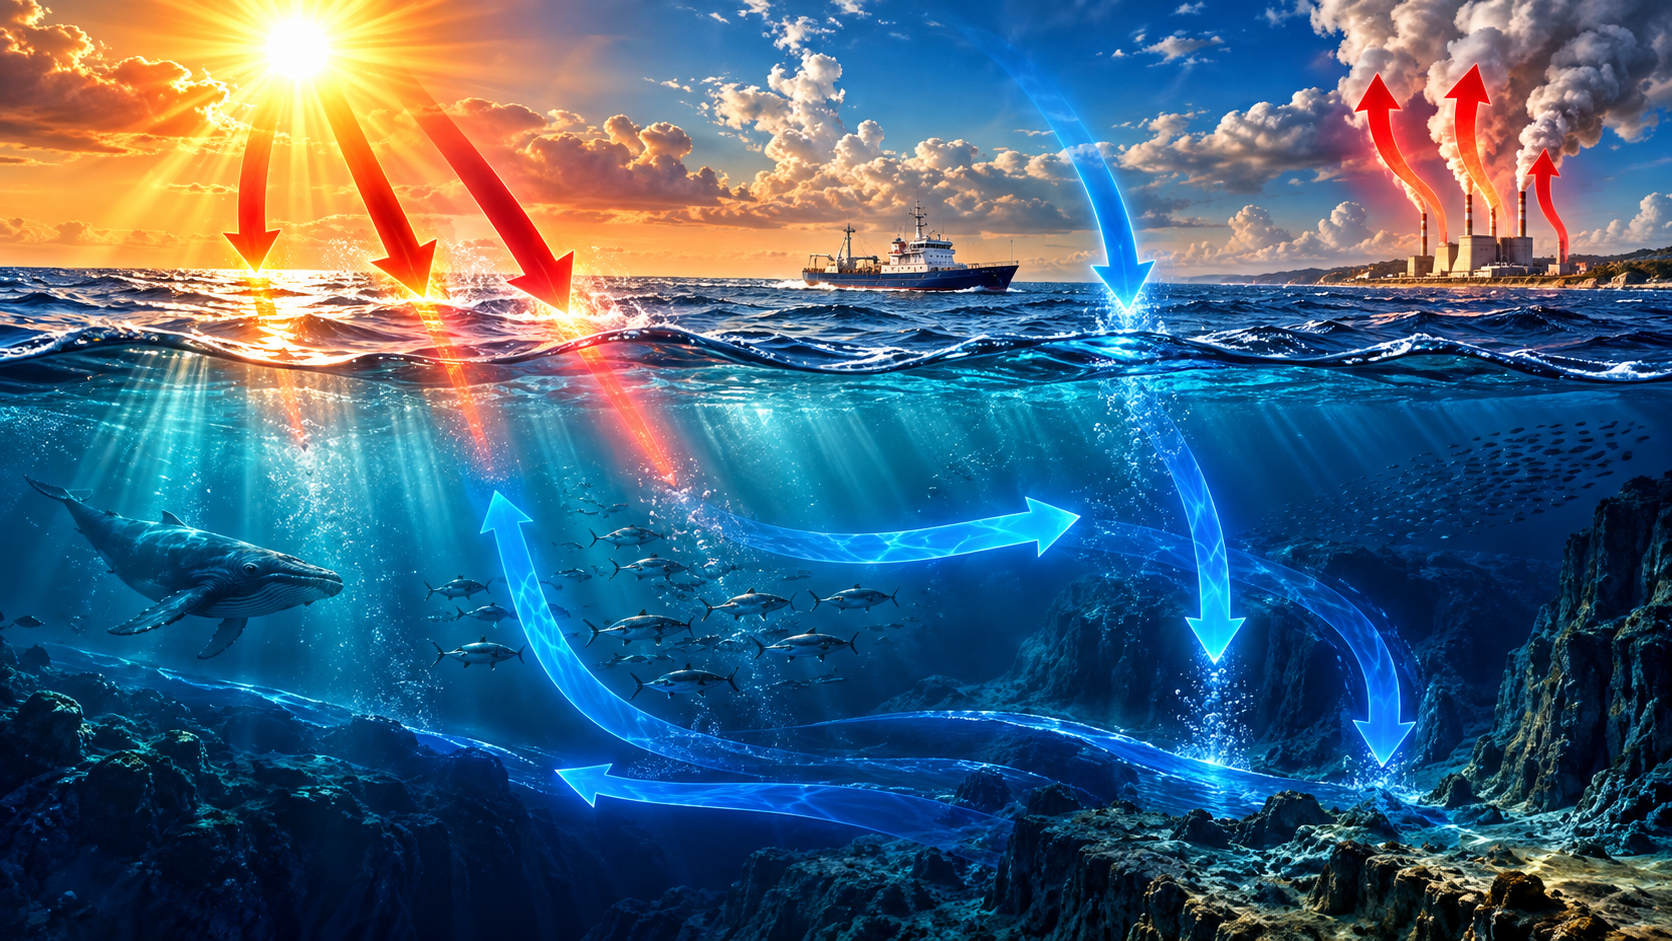
\includegraphics[width=\linewidth]{figures/ch04/ch04-04a-schematic-bad.png}
\end{minipage}\hfill
\begin{minipage}[c]{0.48\linewidth}\centering
\resizebox{\linewidth}{!}{\hbox{\setlength{\linewidth}{\textwidth}% FIG ch04-04b schematic labels (Chinese)
\usetikzlibrary{positioning}
\begin{tikzpicture}
\node[anchor=south west,inner sep=0] (img) at (0,0) {%
  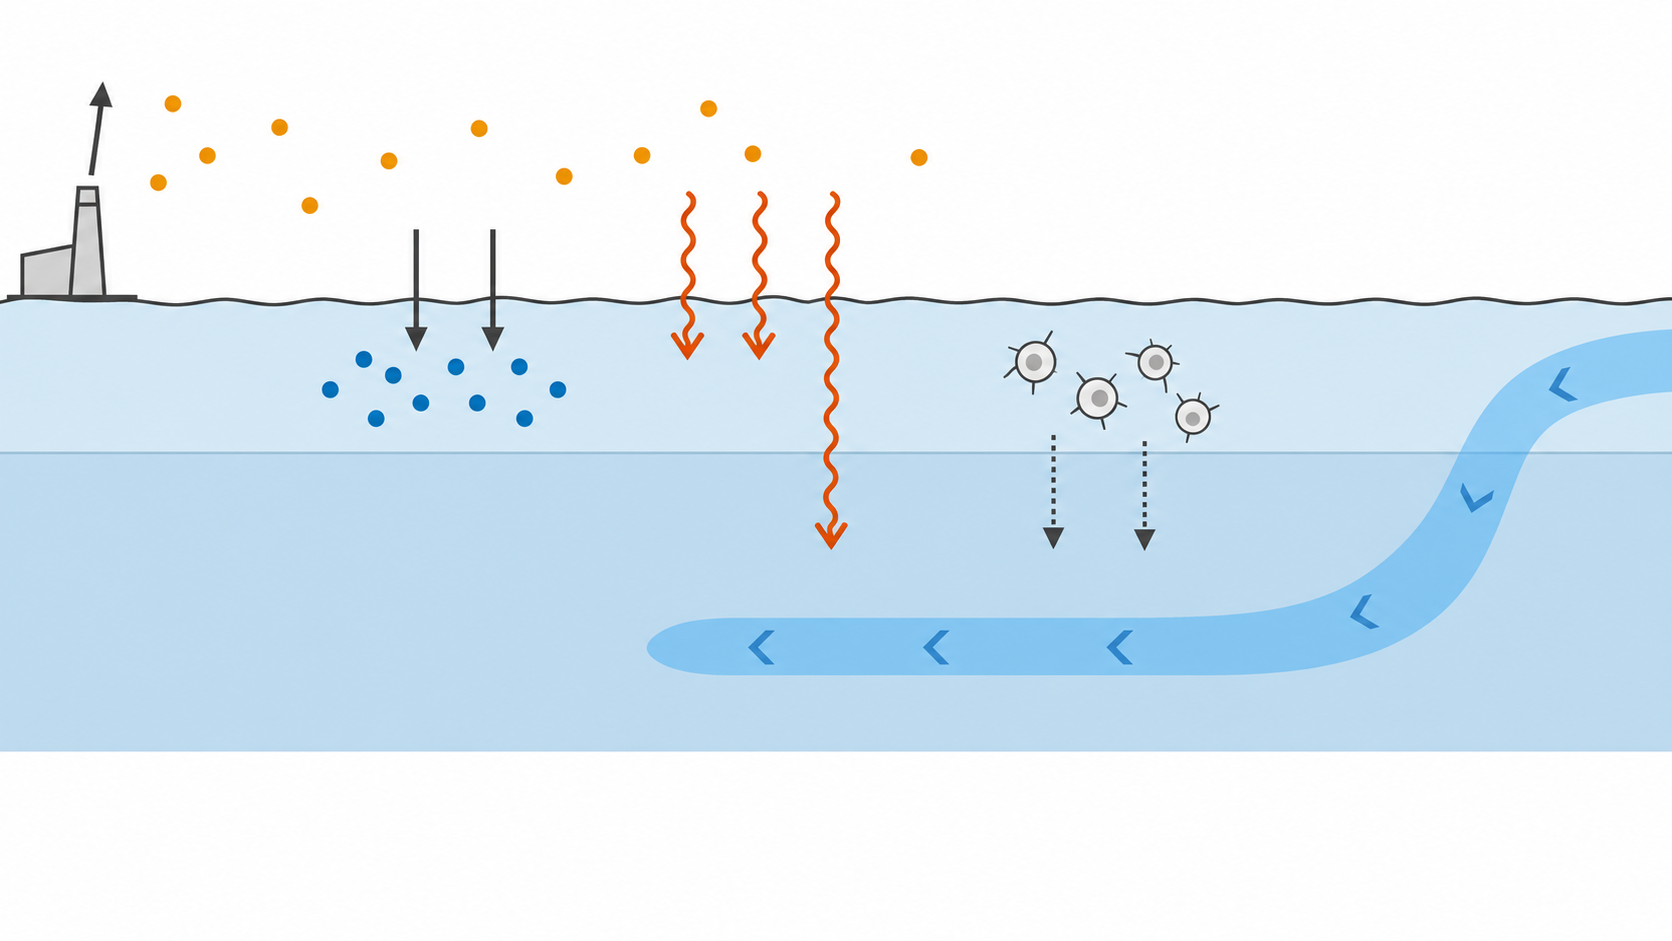
\includegraphics[width=\linewidth]{figures/ch04/ch04-04b-schematic-base.png}};
\begin{scope}[x={(img.south east)},y={(img.north west)},font=\sffamily\small]
  \node at (0.92,0.90) {大气};
  \node at (0.92,0.66) {表层混合层};
  \node at (0.92,0.35) {海洋内部};
  \node[align=left] at (0.06,0.93) {人为排放};
  \node at (0.30,0.88) {CO\textsubscript{2}};
  \node at (0.33,0.70) {海气交换};
  \node at (0.30,0.60) {溶解无机碳};
  \node at (0.55,0.70) {热量吸收};
  \node[align=center] at (0.80,0.45) {水体下沉\\与输运};
  \node at (0.48,0.62) {浮游植物};
  \node[align=center] at (0.48,0.42) {下沉颗粒\\（生物泵）};
  \node[align=center,font=\scriptsize] at (0.50,0.04) {%
    图例：碳通量 / 热通量 / 水体输运 / 下沉颗粒};
\end{scope}
\end{tikzpicture}
}}
\end{minipage}
\caption{示意图也服从同一套视觉语言。左（故意不一致的示范）：3D 光泽渲染、装饰性太阳与船只、模型自行添加的鲸与鱼群，且同色箭头兼表不同过程。右：按规范重画的无文字底图叠加 TikZ 标签，颜色严格留给大气 $\text{CO}_2$（橙）、海水溶解无机碳（蓝）、热（朱红）和水体输运（天蓝），四类过程各用一种箭头形状。两图均为图像模型生成的示意，不按比例。}\label{fig:ch04-04}
\end{figure}

同时要注意右图中“生物泵”的科学边界：浮游植物固碳并以沉降颗粒向深海输出的生物泵，主要转运自然碳循环中的碳；工业革命以来海洋对\textbf{人为 $\text{CO}_2$} 的净吸收，主要由海气气体交换、碳酸盐缓冲化学与物理环流决定（Sabine 等, 2004；Gruber 等, 2019；Fox-Kemper 等, 2023；Canadell 等, 2023）。因此右图将人为 $\text{CO}_2$ 海气交换（左中部深灰实线箭头 $\rightarrow$ 蓝色 DIC 圆点 $\rightarrow$ 右侧天蓝水体下沉带）作为主路径，而将浮游植物与细点线颗粒箭头独立置于中右部，避免画成“人为碳靠浮游植物送入深海”的错误单线链路。

\section{用提示词约束风格，再逐项检查}

立好规范后，用 AI 工具出图时需认清两个客观事实。第一，\textbf{对话式 AI 在协助起草规范或梳理文献时，不了解细分领域惯例，还可能推荐已撤稿文献}——例如利用大气氧碳推算海洋热吸收的一篇 2018 年 \textit{Nature} 论文（Resplandy 等, 2018）已于 2019 年因误差与趋势方法问题撤稿，故所有引文必须经 Crossref 核查撤稿状态。第二，\textbf{\scidraw{} 目前没有跨会话或项目级的全局风格记忆}，界面上的风格预设也不等于你的论文规范。

因此，可靠做法是先把视觉规范保存为带版本号的文档（图~\ref{fig:ch04-02}），提炼出两段可复制的“风格块（style block）”；每次新开会话时先粘贴风格块，生成或修改后再逐项核验。本案例的一页视觉规范（v1）核心条款摘录如下（完整版见配套资料）：

\begin{BookNote}
\textbf{一页视觉规范（v1）核心条款摘录：}
\begin{itemize}
\item \textbf{A.\ 语义色（基于 Okabe–Ito 色板）：}大气碳 \texttt{\#E69F00}（橙，用于 Fig.\ 2a、Fig.\ 4a 大气增长、示意图大气 $\text{CO}_2$ 点，不用于热或海洋量）；海洋碳 \texttt{\#0072B2}（蓝，用于 Fig.\ 2b 海水 $p\text{CO}_2$、Fig.\ 4 海洋碳汇、示意图海水溶解无机碳，不用于水体背景或热）；陆地碳 \texttt{\#009E73}（蓝绿，仅用于 Fig.\ 4 陆地碳汇，不用于浮游植物图标）；热 \texttt{\#D55E00}（朱红，用于 Fig.\ 3 深浅两线与示意图热通量，不用于碳量）；海水 pH \texttt{\#CC79A7}（红紫，专用于 Fig.\ 2c）；人为排放 \texttt{\#3C3C3C}（近黑深灰）；水体输运 \texttt{\#56B4E9}（天蓝，仅用于示意图环流带）；中性灰 \texttt{\#F2F2F2}、\texttt{\#BDBDBD}、\texttt{\#7A7A7A}（背景分区、图标填充、参考线）。
\item \textbf{B.\ 文字层级与尺寸：}Fig.\ 1、2、4 物理宽 $174\ \text{mm}$（双栏），Fig.\ 3 宽 $85\ \text{mm}$（单栏）。面板字母 $8\ \text{pt}$ 粗体小写 \textbf{a}、\textbf{b}、\textbf{c}（左上外侧）；轴标签 $7\ \text{pt}$ 常规；刻度与线端直接标注 $6\ \text{pt}$ 常规（标注与对象同色）；示意图叠加标签对象 $7\ \text{pt}$、过程 $6\ \text{pt}$。图内不放标题，单位统一为括号内 SI 写法（$10^{22}\ \text{J}$、$\text{GtC yr}^{-1}$、$\mu\text{atm}$、ppm）。
\item \textbf{C–E.\ 线型、箭头与图标：}见表~\ref{tab:ch04-lines} 与表~\ref{tab:ch04-arrows}；图标用 $0.75\ \text{pt}$ \texttt{\#3C3C3C} 圆角描边与中性灰填充，无渐变、阴影与高光，禁画太阳、船只、冰山、鱼群。
\item \textbf{F.\ 布局与导出：}坐标轴仅留左下两边（$0.6\ \text{pt}$，刻度朝外），无网格，线端直接标注取代图例框，面板间距 $4\ \text{mm}$；导出矢量 PDF 与高分辨率 PNG，中英文版坐标尺寸一致。
\end{itemize}
\end{BookNote}

在 \scidraw{} 科学可视化（\sdtool{sci-vis}）中每次新开数据图会话时，先粘贴以下数据图风格块：

\begin{Prompt}
Apply this paper-wide figure style exactly (visual spec v1):
- Colours by meaning, no other hues: atmospheric CO2 #E69F00; ocean carbon
  #0072B2; land carbon #009E73; heat #D55E00; seawater pH #CC79A7;
  emissions #3C3C3C; neutral grays #7A7A7A and #BDBDBD only.
- Monthly values: 0.5 pt line in a 50% lighter tint of the series colour.
  Deseasonalized or smoothed values: 1.2 pt solid line. Discrete cruise samples:
  small dots, no connecting line. Uncertainty: band in the series colour at 20%
  opacity, no edge line. Reference lines: 0.5 pt dashed #7A7A7A.
- Sans-serif font. Axis labels 7 pt, tick labels 6 pt, panel letters 8 pt bold
  lowercase (a, b, c) outside the top-left of each axes.
- No title inside the figure, no grid, no legend box: label each series
  directly at its right end in the series colour.
- Only left and bottom axes, 0.6 pt, ticks pointing outward.
- Final size 174 mm wide x 60 mm high.
Keep every data value unchanged: do not smooth, resample, interpolate or drop
rows unless I ask.
\end{Prompt}

\begin{sloppypar}
在提示词绘图（\sdtool{ai-drawing}）或机制图生成（\sdtool{mechanism-figure-generator}）中制作示意图时，则粘贴以下示意图风格块：
\end{sloppypar}

\begin{Prompt}
Flat 2D scientific schematic of ocean heat and carbon uptake, landscape 16:9,
pure white background. ABSOLUTELY NO TEXT: no letters, no words, no numbers, no
symbols, no labels, no legend, no title.
STYLE (paper-wide visual spec v1): flat vector illustration; all outlines 0.75 pt
dark gray #3C3C3C with rounded joins; no gradients, no shadows, no highlights,
no 3D, no glow, no texture, no realistic water. Icons use neutral fills only
(#F2F2F2, #BDBDBD). Colour is used ONLY for the following quantities:
orange #E69F00 = CO2 in the atmosphere; blue #0072B2 = dissolved inorganic
carbon in seawater; vermilion #D55E00 = heat; sky blue #56B4E9 = water
transport. Nothing else may use these colours.
REGIONS (top to bottom): Top 25% atmosphere, white; thin dark gray gently wavy
line at 25% height (sea surface); 25-45% surface mixed layer (#DCEBF5); 45-90%
ocean interior (#C9DEEE); bottom 10% empty white reserved for a legend.
DO NOT DRAW: sun, rays, clouds, ships, fish, ice, land masses other than the
short ground line, sea floor details, coral, bubbles, any charts or data.
\end{Prompt}

\begin{sloppypar}
使用 \sdtool{sci-vis} 时需注意两点：第一，上传数据后的完整性校验（核对哈希、字节数与行数）只证明输入文件未丢行损坏，不证明单位、标度、基准期或配色正确；第二，多轮对话修改极易发生\textbf{风格漂移}——例如追加一句“在 2022 年 12 月加一条细竖线”，工具重写代码时可能悄悄把刻度字号退回默认值或重新加回图例框。因此每次修改后都要复查色值、字号与线型，必要时用历史版本功能回退并重贴风格块。定稿前可用图片检查工具（\sdtool{figure-checker}）筛查分辨率、灰度与色觉风险，但技术检查不代替科学审核。
\end{sloppypar}

\section{案例：四张图从各自为政到一套}

下面回到小宋的论文，按“材料清点 $\rightarrow$ 规范制定 $\rightarrow$ 示意图与数据图重绘 $\rightarrow$ 整套对照与核验”走完整个改造过程。

\textbf{第一步：清点原始材料与数据处理规则。}四套公开数据集于 2026 年 10 月 29 日下载固化，字段、单位、质控规则与引用要求汇总于表~\ref{tab:ch04-sources}。在图 2 中，莫纳罗亚大气 $\text{CO}_2$ 为\textbf{干空气摩尔分数}（ppm），而 ALOHA 站表层海水 $p\text{CO}_2$ 为现场温盐下由 DIC 与总碱度计算的\textbf{分压}（$\mu\text{atm}$）；两者数值虽都在 $300\text{--}430$ 附近，但物理量纲不同，不能硬叠在同一纵轴上，故拆为 \textbf{a}、\textbf{b}、\textbf{c} 三个并排面板。

\begin{table}[htbp]\centering\scriptsize
\setlength{\tabcolsep}{2.5pt}
\renewcommand{\arraystretch}{1.12}
\caption{主案例四张图使用的公开数据源、质控规则与引用要求（2026 年 10 月 29 日下载）。}\label{tab:ch04-sources}
\begin{tabularx}{\linewidth}{@{}>{\raggedright\arraybackslash}p{20mm}>{\raggedright\arraybackslash}p{24mm}>{\raggedright\arraybackslash}p{18mm}Y>{\raggedright\arraybackslash}p{26mm}@{}}
\toprule
\textbf{数据集（图）} & \textbf{文件与规模} & \textbf{字段与单位} & \textbf{数据处理与质控规则} & \textbf{许可与引用要求} \\
\midrule
莫纳罗亚大气 $\text{CO}_2$（Fig.\ 2a） & \path{co2_mm_mlo.csv}；823 行（1958-03 至 2026-09） & \texttt{average}、\path{deseasonalized}（ppm） & 跳过 \texttt{\#} 注释行；确认无 $-99.99$ 缺测（均值 $361.44\ \text{ppm}$）；不自行平滑；标出 2022-12 至 2023-07 火山喷发改在 Maunakea 观测 & 美国政府公开数据；同时致谢 NOAA GML 与 Scripps（Keeling） \\
HOT 表层海水碳酸盐（Fig.\ 2b, c） & \path{HOT_surface_CO2.txt}；355 行（1988-10-31 起） & \path{pCO2calc_insitu}（$\mu\text{atm}$）、\path{pHcalc_insitu} & 跳过前 8 行；将 $\le -900$（缺测码 $-999$）置为 \texttt{NaN}，得有效记录各 346 条；两位年份按 1988–2026 解析；pH 标度需核对 \path{HOT_surface_CO2_readme.pdf} 填入图注 & 按文件头引用 Dore 等（2009）；未见显式开放许可，重绘须规范引用 \\
全球海洋热含量距平（Fig.\ 3） & \path{pent_h22-w0-700m.dat} 与 \texttt{2000m.dat}；各 67 行 & \texttt{YEAR}（1957.5–2023.5）、\texttt{WO}、\texttt{WOse}（$10^{22}\ \text{J}$） & 两深度年份行数一致（均值 $3.84$ 与 $5.09\times 10^{22}\ \text{J}$）；阴影画 $\text{WO} \pm 1\ \text{WOse}$；距平基准期需核对 NCEI 说明页后填入图注 & NOAA NCEI 美国政府作品；引用 Levitus 等（2012） \\
全球碳收支 GCB 2025（Fig.\ 4） & \path{GlobalCarbonBudget_v2025.xlsx}；66 行（1959–2024） & 排放与三大碳汇（$\text{GtC yr}^{-1}$） & 读 \texttt{Global Carbon Budget} 表（第 22 行表头）；总排放 = 化石 + 土地利用；绘平均不确定性（海洋 $\pm 0.4$、陆地 $\pm 0.5$）；面板 b 由作者算海洋占比（均值 $27.01\%$）与 10 年滑动平均 & 遵循 Fair Use 声明；引用 Friedlingstein 等（2026）并致谢 GCP \\
\bottomrule
\end{tabularx}
\end{table}

\textbf{第二步：重绘示意图（Fig.\ 1）并核查生成偏差。}为了看清提示词如何直接决定示意图是否合群，先看图~\ref{fig:ch04-04} 左图（不一致反例）所使用的提示词：

\begin{Prompt}
A glossy, highly polished 3D illustration of an ocean cross-section for a
climate science paper, landscape 16:9. Photorealistic blue waves on top, a
bright sun with radiating rays in a gradient orange-to-blue sky, a small ship
on the surface, shiny glass-like water with caustics and depth of field.
Thick glowing red 3D arrows go from the sky into the water and also from a
factory into the sky; thick glowing blue 3D arrows curve through the water and
also go from the air into the water. Dramatic lighting, lens flare, strong
shadows, saturated colors. No text, no letters, no numbers, no labels.
\end{Prompt}

这段追求“3D 光泽、写实波浪、戏剧性光效”的提示词直接造就了左图的三大硬伤：红箭头同时画在工厂烟囱和太阳光束上，蓝箭头同时画在海气界面和深海环流上，且由于未设排除清单，模型顺手在水下塞进了鲸、鱼群和礁石。

相反，重绘右图时，我们在第 4.5 节的示意图风格块之后接上下列七项对象与过程指令（完整提示词见本书仓库 \texttt{cases/} 目录）：

\begin{Prompt}
OBJECTS AND PROCESSES (draw exactly these, nothing else):
1. Top-left: one simple factory chimney icon in neutral gray on a short ground
   line, with one straight dark gray arrow (filled head) rising into the air.
2. Atmosphere: about 12 small orange dots scattered in the left and middle.
3. Air-sea gas exchange: two straight dark gray arrows with filled heads, going
   down from the atmosphere through the sea surface into the mixed layer.
4. Mixed layer: about 10 small blue #0072B2 dots near the two arrows.
5. Heat uptake: three vermilion wavy arrows with open V-shaped heads, going down
   into the mixed layer; the rightmost continues into the ocean interior.
6. Water transport: on the right, one broad semi-transparent sky-blue band from
   the mixed layer curving down into the interior and running leftward, with
   chevron marks pointing along the flow.
7. Biological pump: 3-4 small round phytoplankton cell icons (neutral fill, gray
   outline) in the mixed layer, and two dotted dark gray arrows pointing down.
Leave white space around each process for labels.
\end{Prompt}

同一提示词连续生成三次候选底图后，逐张核验可见：
\begin{itemize}
\item \textbf{第 1 次候选（因流向自相矛盾淘汰）：}主要对象与数量均符合，但右侧天蓝色水体输运宽带内上、中段的人字纹指向右上，底段却指向左，同一流带内流向迎头相撞，故淘汰。
\item \textbf{第 2 次候选（选用为图~\ref{fig:ch04-04} 右图底图）：}七项对象与四类箭头齐备，右侧输运宽带内人字纹一致顺流指向左下与正左，无文字且无太阳、轮船、鱼群等禁止对象。
\item \textbf{第 3 次候选（落选）：}流向一致，但给浮游植物细胞加了未要求的鞭毛状突起，点线箭头偏粗，且第二色盲模拟下朱红热箭头与内部背景的最小亮度对比（$2.17:1$）略低于第 2 次候选（$2.36:1$）。
\end{itemize}

对选用的第 2 次候选底图做像素复查，仍可发现三处真实偏差：（1）\textbf{色值仅近似命中}——各对象 RGB 中位数实测为大气橙点 \texttt{\#ED9106}（规范 \texttt{\#E69F00}）、海水蓝点 \texttt{\#0571BA}（规范 \texttt{\#0072B2}）、热箭头 \texttt{\#DD4E0A}（规范 \texttt{\#D55E00}）、碳箭头 \texttt{\#3F3F40}（规范 \texttt{\#3C3C3C}），全图精确命中指定 HEX 的像素数为零，且水层与图标仍有轻微明暗纹理；（2）\textbf{分区比例与对象位置偏移}——海面、混合层底界与底部留白起点实测约为 $32\%$、$48\%$、$80\%$（规范为 $25\%$、$45\%$、$90\%$），且 4 个浮游植物细胞偏在混合层中右部，导致按预设中央坐标（横坐标 $0.48$）叠加的“浮游植物”标签落在细胞群左侧空白处（图~\ref{fig:ch04-04} 右），定稿前需在 TikZ 层右移校准；（3）\textbf{原生分辨率限制}——在 $174\ \text{mm}$ 宽度下原生有效分辨率约 $244\ \text{ppi}$，且无矢量可编辑线宽。这直观说明生成式底图只是近似遵循规范，后期取色核查与标签位置微调必不可少。

\textbf{第三步：按规范重绘三张数据图（Fig.\ 2–4）。}共享同一视觉规范常数重绘后（修改对照见表~\ref{tab:ch04-revisions}）：

\begin{figure}[htbp]\centering
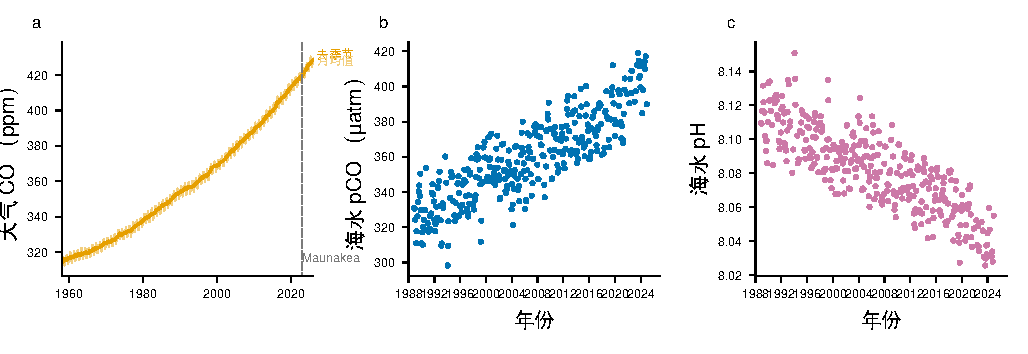
\includegraphics[width=\linewidth]{figures/ch04/ch04-05-fig2-carbonate-zh.pdf}
\caption{按规范重绘的论文 Fig.\ 2：大气 $\text{CO}_2$ 与北太平洋亚热带表层海水碳酸盐系统的变化。（a）莫纳罗亚站大气 $\text{CO}_2$ 月均值（细浅橙线）与去季节值（粗橙线）；1958 年 3 月至 1974 年 4 月数据来自 Scripps，2022 年 12 月至 2023 年 7 月因火山喷发改在 Maunakea 观测（灰色细虚线）。（b）HOT ALOHA 站表层海水 $p\text{CO}_2$（由 DIC 与总碱度计算的现场值，每点一个航次）。（c）同站表层海水 pH（现场温度计算值，标度待核实）。数据：NOAA GML 与 Scripps；HOT（Dore 等, 2009），2026 年 10 月 29 日下载。}\label{fig:ch04-05}
\end{figure}

在图~\ref{fig:ch04-05}（论文 Fig.\ 2）中，面板 \textbf{a} 用橙色（\texttt{\#E69F00}）区分月均值细浅线与去季节粗线，并标出 Maunakea 换站虚线；面板 \textbf{b} 用海洋碳蓝色（\texttt{\#0072B2}）、面板 \textbf{c} 用红紫色（\texttt{\#CC79A7}）将 346 个有效航次画成无连线圆点。$100\%$ 尺寸复查也揭示了三处待微调细节：面板 \textbf{a} 右上末端“去季节”与“月均值”因终值接近而上下重叠，需加纵向偏移；面板 \textbf{b}、\textbf{c} 横轴 4 年间隔刻度略挤，宜改为 10 年一标；纵轴标签下标 $2$ 需补回显式数学下标。

\begin{figure}[htbp]\centering
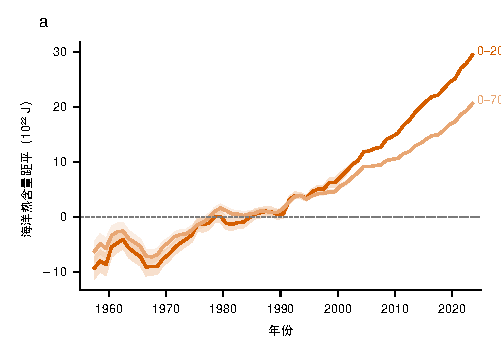
\includegraphics[width=0.58\linewidth]{figures/ch04/ch04-06-fig3-ohc-zh.pdf}
\caption{按规范重绘的论文 Fig.\ 3：全球海洋热含量距平。$0\text{--}700\ \text{m}$（浅朱红）与 $0\text{--}2000\ \text{m}$（深朱红）水层五年平均热含量距平，单位 $10^{22}\ \text{J}$；横轴为五年窗口中点年份；阴影为 NCEI 提供的 $\pm 1$ 标准误；灰虚线为零线。距平基准期需核对 NCEI 文档后注明。数据：NOAA NCEI（Levitus 等, 2012 方法及更新）。}\label{fig:ch04-06}
\end{figure}

在图~\ref{fig:ch04-06}（论文 Fig.\ 3，单栏宽 $85\ \text{mm}$）中，两条曲线统一归入代表热量的朱红色相（\texttt{\#D55E00}），靠深浅明度、$\pm 1\ \text{WOse}$ 阴影带和右端直接标注区分，清晰展现海洋上层与中深层持续吸热的趋势（von Schuckmann 等, 2023）。复查可见右端直接标注“$0\text{--}2000\ \text{m}$”和“$0\text{--}700\ \text{m}$”因右边距预留不足被裁去末尾字符，提示使用线端标注时必须同步放宽横轴上限或右页边距。

\begin{figure}[htbp]\centering
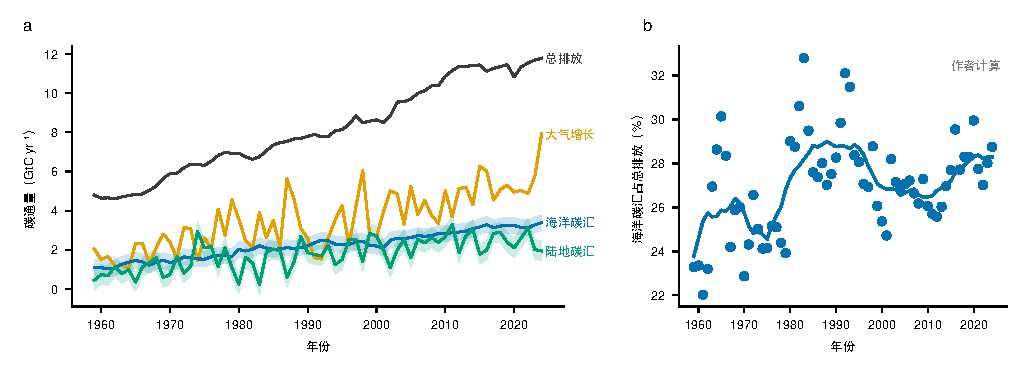
\includegraphics[width=\linewidth]{figures/ch04/ch04-07-fig4-budget-zh.pdf}
\caption{按规范重绘的论文 Fig.\ 4：人为 $\text{CO}_2$ 排放的去向。（a）化石燃料与土地利用变化总排放（深灰）以及大气增长（橙）、海洋碳汇（蓝）、陆地碳汇（蓝绿），单位 $\text{GtC yr}^{-1}$；阴影为 GCB 给出的平均不确定性（海洋 $\pm 0.4$、陆地 $\pm 0.5\ \text{GtC yr}^{-1}$）。（b）海洋碳汇占总排放的比例（作者据 GCB 数据计算；点为年值，线为 10 年居中滑动平均）。收支不平衡项与水泥碳化汇未画出。数据：Global Carbon Budget 2025（Friedlingstein 等, 2026）。}\label{fig:ch04-07}
\end{figure}

在图~\ref{fig:ch04-07}（论文 Fig.\ 4）中，面板 \textbf{a} 将原先因收支不平衡项而穿越黑线的 \texttt{jet} 堆叠面积图改为四条语义色实线配不确定性带，右端同色标签互不重叠；面板 \textbf{b} 用海洋碳蓝色（\texttt{\#0072B2}）画出年值散点与 10 年居中滑动平均线（全期均值约 $27.0\%$），并在右上角注明“作者计算”。

\begin{table}[htbp]\centering\footnotesize
\setlength{\tabcolsep}{3pt}
\renewcommand{\arraystretch}{1.15}
\caption{从不一致初稿（图~\ref{fig:ch04-01}）到规范重绘稿（图~\ref{fig:ch04-04}–\ref{fig:ch04-07}）的修改记录。}\label{tab:ch04-revisions}
\begin{tabularx}{\linewidth}{@{}>{\raggedright\arraybackslash}p{14mm}Y>{\raggedright\arraybackslash}p{20mm}>{\raggedright\arraybackslash}p{36mm}@{}}
\toprule
\textbf{对象图} & \textbf{具体修改内容} & \textbf{依据条款} & \textbf{核对方式与实测复查记录} \\
\midrule
Fig.\ 1 & 删去 3D 光泽、太阳、船只、鲸与鱼群；改为二维分层底图；四类过程按表~\ref{tab:ch04-arrows} 箭头重画；叠加 TikZ 标签 | 规范 A、D、E & 3 次候选中淘汰流向冲突的第 1 次，选第 2 次；记录实测 HEX 近似与浮游植物偏右，待微调标签坐标 \\
Fig.\ 2a & 双红粗线改为 \texttt{\#E69F00} 橙色（月均值 $0.5\ \text{pt}$ 浅线 + 去季节 $1.2\ \text{pt}$ 实线）；补 Maunakea 灰虚线 & 规范 A、C & 取色器核对 HEX；末端两标签轻微重叠，需加纵向偏移 \\
Fig.\ 2b, c & 绿、蓝折线改为 \texttt{\#0072B2}（海洋碳）与 \texttt{\#CC79A7}（pH）的 $2.5\ \text{pt}$ 无连线圆点 & 规范 A、C & 核对 346 个有效航次点无连线；横轴 4 年刻度略挤，宜改为 10 年间隔 \\
Fig.\ 3 & 红绿双线改为朱红（\texttt{\#D55E00}）深浅两色；加 $\pm 1\ \text{WOse}$ 带与零线；去掉 \texttt{1e23} 偏移 & 规范 A、B、C & 第二色盲模拟下可分（图~\ref{fig:ch04-03}）；右端标注被裁半词，需扩右边距 \\
Fig.\ 4 & 彩虹堆叠图改为四条语义色实线 + 误差带；新增面板 b 海洋汇占比并标“作者计算” & 规范 A、B、C & 66 年数值与原表逐年一致；四条线端直接标注清晰 \\
全部四图 & 统一无衬线字体与 8/7/6 pt 层级；面板字母改为左上粗体小写 \textbf{a}–\textbf{c}；删图内标题与网格 & 规范 B、F & 100\% 尺寸 PDF 量字号；排查出上下标字符缺字问题 \\
\bottomrule
\end{tabularx}
\end{table}

\textbf{第四步：整套拼版对照、规范图注与全表核验。}将修改后的四张图按与图~\ref{fig:ch04-01} 相同的 $2 \times 2$ 版式拼成总览（图~\ref{fig:ch04-08}），底部附上六色语义提示条。

\begin{figure}[htbp]\centering
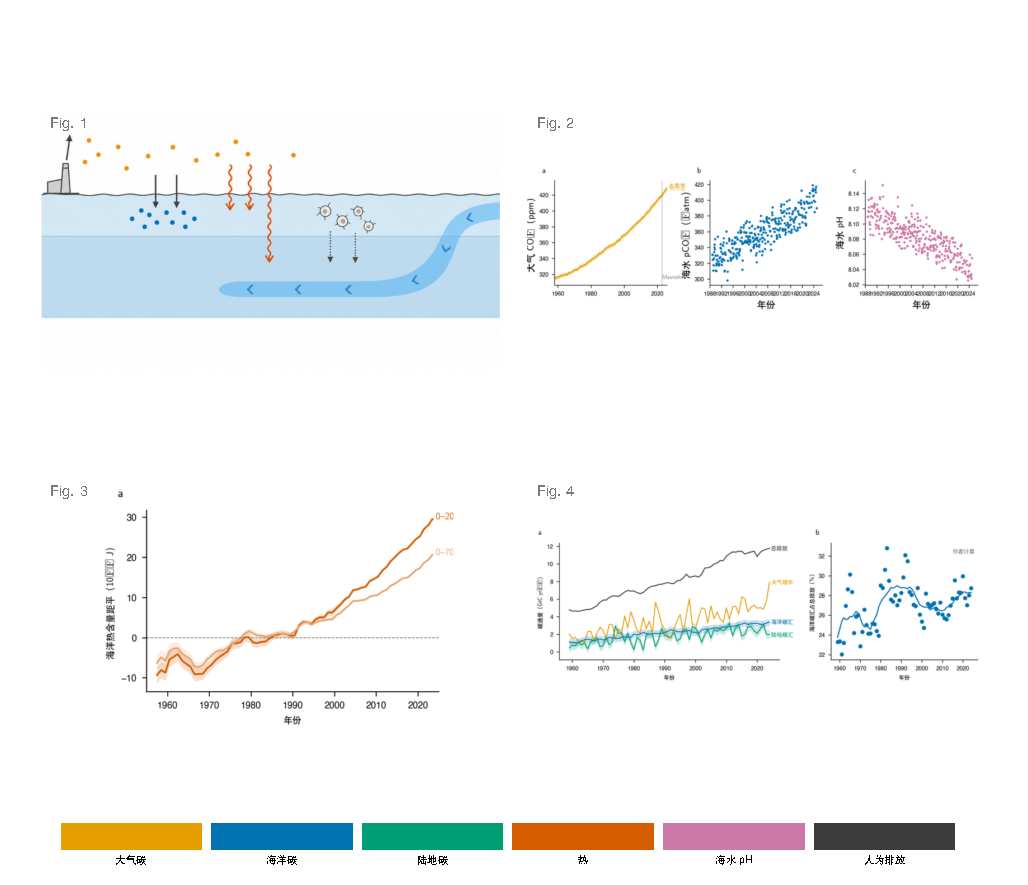
\includegraphics[width=\linewidth]{figures/ch04/ch04-08-consistent-set-zh.pdf}
\caption{按同一页视觉规范修改后的四张论文图。每种颜色在全文中只代表一类物理量或碳库（底部色条），字体、字号、面板编号、线型与箭头形状统一。与图~\ref{fig:ch04-01} 相比，底层数据完全相同，只改变了视觉语言。}\label{fig:ch04-08}
\end{figure}

对比图~\ref{fig:ch04-08} 与图~\ref{fig:ch04-01}，读者无需反复查阅图例框，就能顺着橙色（大气碳）串起 Fig.\ 1、Fig.\ 2a 与 Fig.\ 4a，顺着蓝色（海洋碳）串起 Fig.\ 1、Fig.\ 2b 与 Fig.\ 4a/b，顺着朱红色（热量）串起 Fig.\ 1 与 Fig.\ 3。除图~\ref{fig:ch04-05}–\ref{fig:ch04-07} 已给出的图注外，论文 Fig.\ 1 的完整图注定稿如下，四张图的跨图总核验记录见表~\ref{tab:ch04-verify}。

\begin{BookNote}
\textbf{论文图 1 图注定稿：} \textbf{图 1　海洋吸收热量与人为 $\text{CO}_2$ 的主要途径示意。} 大气中增加的热量经海气界面进入表层混合层（波浪箭头），并随混合与水体下沉输送到海洋内部（浅蓝带）。人为排放的 $\text{CO}_2$ 经海气交换溶入表层海水（直线箭头），使海水 $p\text{CO}_2$ 升高、pH 降低，并同样随水体输运进入内部。浮游植物固定碳并以下沉颗粒形式输出（点线箭头），这一生物泵主要转运自然碳循环中的碳；人为 $\text{CO}_2$ 的吸收主要由海气交换、海水化学与环流决定。示意图，不按比例；省略了区域差异、季节变化、海冰、沉积物与河流输入。依据 Sabine 等（2004）、Gruber 等（2019）与 IPCC AR6 第一工作组第 5、9 章整理。
\end{BookNote}

\begin{table}[htbp]\centering\footnotesize
\setlength{\tabcolsep}{3pt}
\renewcommand{\arraystretch}{1.15}
\caption{主案例四张论文图的跨图总核验记录。}\label{tab:ch04-verify}
\begin{tabularx}{\linewidth}{@{}>{\raggedright\arraybackslash}p{38mm}YYYY@{}}
\toprule
\textbf{核验项目} & \textbf{Fig.\ 1} & \textbf{Fig.\ 2} & \textbf{Fig.\ 3} & \textbf{Fig.\ 4} \\
\midrule
语义色符合规范 A（跨图同色同义） & 通过（色值近似） & 通过 & 通过 & 通过 \\
色觉模拟与灰度下同面板可分 & 靠形状冗余可分 & 分面板无冲突 & 通过（图~\ref{fig:ch04-03}） & 通过（加直接标注） \\
100\% 尺寸字号符合 8/7/6 pt & 通过 & 通过 & 通过 & 通过 \\
面板字母与单位一致，无缺字裁切 & 浮游植物标签待右移 & 下标 2 与末端重叠待修 & 右端标签被裁待扩边距 & 上标负号遗失待修 \\
线型与箭头符合表~\ref{tab:ch04-lines}、\ref{tab:ch04-arrows} & 通过 & 通过 & 通过 & 通过 \\
起止年份与行数同原文件一致 & — & 823 行 / 346 点 & 67 行（双深度一致） & 66 行（1959–2024） \\
作者计算项与不确定性已入图注 & — & pH 标度待核文档 & 基准期待核文档 & 已标“作者计算” \\
数据引用完整，领域同行复核 & 待海洋同行复核 & 已含 NOAA / Scripps / HOT & 已含 NCEI / Levitus & 已含 GCB 2025 \\
\bottomrule
\end{tabularx}
\end{table}

\section{AI 在这一步能做什么与不能做什么}

在建立并执行整篇论文视觉语言的过程中，AI 工具与作者的职责边界汇总于表~\ref{tab:ch04-01}。

\begin{table}[htbp]\centering\footnotesize
\setlength{\tabcolsep}{3pt}
\renewcommand{\arraystretch}{1.15}
\caption{在建立整篇论文视觉语言环节，AI 能做什么、不能做什么及作者要核对的内容。}\label{tab:ch04-01}
\begin{tabularx}{\linewidth}{@{}>{\raggedright\arraybackslash}p{18mm}YYY@{}}
\toprule
\textbf{环节} & \textbf{AI 能做} & \textbf{AI 不能做 / 不可靠} & \textbf{作者要核对} \\
\midrule
起草规范 & 对话式 AI 可根据图清单提出语义色分配、字号层级的初稿，并推荐色觉友好的色板 & 不知道你所在领域的颜色惯例和目标期刊要求；可能推荐不存在或已撤稿的“依据” & 规范条款逐条确认；引用用 Crossref 查 DOI 与撤稿状态 \\
跨图记忆 & — & \scidraw{} 目前没有项目级风格设置，不会在不同会话、不同工具之间记住你的规范 & 规范保存为文档；每次新会话粘贴风格块 \\
数据图套用样式 & \sdtool{sci-vis} 可按风格块生成图，并在对话中逐项修改；可恢复历史版本 & 多轮修改后可能悄悄改回默认颜色、字号或加回图例；“已按规范”的回答不等于做到了 & 每次修改后取色、量字号、对线型表；保存每个满意版本 \\
数据完整性 & \sdtool{sci-vis} 对上传的源数据做哈希、字节数与行数校验 & 校验只证明输入没丢，不证明单位、标度、基准期或计算正确 & 起止时间、行数、单位、基准期对照原始文件与数据说明 \\
示意图套用样式 & 绘图与参考图修改可按风格块生成扁平示意并调整颜色 & 色值、线宽只能近似；可能出现局部流向矛盾或加入未要求的对象 & 多次候选比选；逐色取色；对照箭头表；删去多余对象并校准标签位置 \\
色觉与技术检查 & \sdtool{figure-checker} 可做格式、分辨率、色彩、灰度与色觉风险等技术检查 & 不审核科学内容；色觉模拟是近似，不能代替询问色觉差异读者 & 用模拟 + 灰度 + 至少一位读者确认；科学内容另行核验 \\
图注 & \sdtool{figure-legend} 可根据图片起草图注 & 不知道数据来源、处理、基准期；不得让它补写这些信息 & 来源、单位、作者计算项、不确定性含义由作者填写 \\
\bottomrule
\end{tabularx}
\end{table}

\section{本章检查清单}

\begin{itemize}
\item 我有一页书面的视觉规范，并给它标了版本号。
\item 每个语义色只表示一类量，每类量只用一个语义色；跨所有图核对过。
\item 语义色不超过 6–7 个，其余元素用灰。
\item 同一面板中的颜色在色觉模拟和灰度下仍可区分，或另有形状、线型、直接标注作冗余。
\item 连续变量用感知均匀的顺序或发散色图，没有使用彩虹色图。
\item 字号在最终印刷尺寸下量过：面板字母、轴标签、刻度、注释四级一致。
\item 全文一种字体；中英文版位置与字号一致，且检查了上下标与特殊字符无缺字。
\item 单位写法、面板字母写法在所有图中相同。
\item 每种线型、每种箭头形状只有一个含义，图例中定义一次。
\item 图标用中性色，没有未讨论的装饰对象。
\item 风格块在每次新会话中重新粘贴，每次修改后都复查了颜色和字号。
\item 数据图的来源、下载日期、处理方式、作者计算项都写进了图注。
\item 我把所有图按最终尺寸放在一页上看过一次。
\end{itemize}

\section{练习}

\begin{enumerate}
\item \textbf{（纸笔：给你的论文分配语义色）} 列出你正在写的论文（或一篇你熟悉的论文）中所有图里出现的“量”或“类别”。（a）把它们合并成不超过 6 类；（b）为每类指定一个 Okabe–Ito 色并写出“用于 / 不用于”；（c）找出现有图中违反这张表的地方，至少三处，写出修改方案；（d）说明你的学科有没有必须遵守的颜色惯例（例如温度暖色、降水蓝绿），你的分配是否与之冲突。
\item \textbf{（色觉与灰度检查）} 选你论文中的一张数据图。（a）导出 PNG，用 \scidraw{} 图片检查（\sdtool{figure-checker}）查看色觉风险与灰度结果，或用 \texttt{colorspacious} 自行模拟三种色觉差异；（b）指出哪一对颜色在模拟下最难区分；（c）在不增加新色相的前提下，用明度、线型或直接标注解决这个问题；（d）说明为什么模拟结果不能代替询问真实读者。
\item \textbf{（\scidraw{} 实操：同一份数据，用风格块约束）} 从 NOAA GML 下载 \texttt{co2\_mm\_mlo.csv}，去掉以 \texttt{\#} 开头的注释行，另存为纯 CSV（记录 SHA-256 与行数）。（a）在 \scidraw{} 科学可视化（\sdtool{sci-vis}）中上传该文件，只说“画大气 $\text{CO}_2$ 时间序列”，保存结果；（b）新开会话，上传同一文件，粘贴本章的数据图风格块再提出同样要求；（c）再追加两轮修改（例如“把月均值改成更浅”“在 2022 年 12 月处加一条细竖线”），检查每轮后颜色与字号是否仍符合规范，记录任何漂移；（d）对比（a）（b）（c）三版，交一份逐项核对表（颜色、字号、线型、标注、数据行数），并写出致谢 NOAA GML 与 Scripps 的一句话。（注：本章示例图由图像模型与配套脚本生成，提示词与生成记录见本书仓库。）
\end{enumerate}

\section*{参考文献}

{\sloppy
\begin{itemize}
\item Brewer CA. ColorBrewer 2.0: Color advice for cartography. \url{https://colorbrewer2.org}
\item Canadell JG, Monteiro PMS, Costa MH, Cotrim da Cunha L, Cox PM, Eliseev AV, Henson S, Ishii M, Jaccard S, Koven C, Lohila A, Patra PK, Piao S, Rogelj J, Syampungani S, Zaehle S, Zickfeld K. Global carbon and other biogeochemical cycles and feedbacks. In: \textit{Climate Change 2021: The Physical Science Basis. Contribution of Working Group I to the Sixth Assessment Report of the Intergovernmental Panel on Climate Change}. Cambridge University Press; 2023:673--816. doi:10.1017/9781009157896.007
\item Crameri F, Shephard GE, Heron PJ. The misuse of colour in science communication. \textit{Nature Communications}. 2020;11:5444. doi:10.1038/s41467-020-19160-7
\item Dore JE, Lukas R, Sadler DW, Church MJ, Karl DM. Physical and biogeochemical modulation of ocean acidification in the central North Pacific. \textit{Proceedings of the National Academy of Sciences}. 2009;106(30):12235--12240. doi:10.1073/pnas.0906044106
\item Fox-Kemper B, Hewitt HT, Xiao C, Aðalgeirsdóttir G, Drijfhout SS, Edwards TL, Golledge NR, Hemer M, Kopp RE, Krinner G, Mix A, Notz D, Nowicki S, Nurhati IS, Ruiz L, Sallée J-B, Slangen ABA, Yu Y. Ocean, cryosphere and sea level change. In: \textit{Climate Change 2021: The Physical Science Basis. Contribution of Working Group I to the Sixth Assessment Report of the Intergovernmental Panel on Climate Change}. Cambridge University Press; 2023:1211--1362. doi:10.1017/9781009157896.011
\item Friedlingstein P, O'Sullivan M, Jones MW, et al. Global Carbon Budget 2025. \textit{Earth System Science Data}. 2026;18:3211--3288. doi:10.5194/essd-18-3211-2026
\item Gruber N, Clement D, Carter BR, Feely RA, van Heuven S, Hoppema M, Ishii M, Key RM, Kozyr A, Lauvset SK, Lo Monaco C, Mathis JT, Murata A, Olsen A, Perez FF, Sabine CL, Tanhua T, Wanninkhof R. The oceanic sink for anthropogenic $\text{CO}_2$ from 1994 to 2007. \textit{Science}. 2019;363(6432):1193--1199. doi:10.1126/science.aau5153
\item Krzywinski M. Elements of visual style. \textit{Nature Methods}. 2013;10(5):371. doi:10.1038/nmeth.2444
\item Levitus S, Antonov JI, Boyer TP, Baranova OK, Garcia HE, Locarnini RA, Mishonov AV, Reagan JR, Seidov D, Yarosh ES, Zweng MM. World ocean heat content and thermosteric sea level change (0--2000 m), 1955--2010. \textit{Geophysical Research Letters}. 2012;39:L10603. doi:10.1029/2012GL051106
\item NOAA Global Monitoring Laboratory. Trends in Atmospheric Carbon Dioxide (Mauna Loa, Hawaii) and Scripps Institution of Oceanography $\text{CO}_2$ Program. \url{https://gml.noaa.gov/ccgg/trends/} and \url{https://scrippsco2.ucsd.edu/}
\item Nuñez JR, Anderton CR, Renslow RS. Optimizing colormaps with consideration for color vision deficiency to enable accurate interpretation of scientific data. \textit{PLOS ONE}. 2018;13(8):e0199239. doi:10.1371/journal.pone.0199239
\item Okabe M, Ito K. Color Universal Design (CUD): How to make figures and presentations that are friendly to colorblind people. 2008. \url{https://jfly.uni-koeln.de/color/}
\item Rougier NP, Droettboom M, Bourne PE. Ten simple rules for better figures. \textit{PLoS Computational Biology}. 2014;10(9):e1003833. doi:10.1371/journal.pcbi.1003833
\item Sabine CL, Feely RA, Gruber N, Key RM, Lee K, Bullister JL, Wanninkhof R, Wong CS, Wallace DWR, Tilbrook B, Millero FJ, Peng T-H, Kozyr A, Ono T, Rios AF. The oceanic sink for anthropogenic $\text{CO}_2$. \textit{Science}. 2004;305(5682):367--371. doi:10.1126/science.1097403
\item von Schuckmann K, Minière A, Gues F, Cuesta-Valero FJ, Kirchengast G, Adusumilli S, Straneo F, et al. Heat stored in the Earth system 1960--2020: where does the energy go? \textit{Earth System Science Data}. 2023;15(4):1675--1709. doi:10.5194/essd-15-1675-2023
\item Wong B. Points of view: Color coding. \textit{Nature Methods}. 2010;7(8):573. doi:10.1038/nmeth0810-573
\item Wong B. Points of view: Typography. \textit{Nature Methods}. 2011;8(4):277. doi:10.1038/nmeth0411-277
\item Wong B. Points of view: Color blindness. \textit{Nature Methods}. 2011;8(6):441. doi:10.1038/nmeth.1618 (Author Correction: \textit{Nature Methods}. 2023;20:1442. doi:10.1038/s41592-023-01974-0)
\end{itemize}
\par}
